%!TEX program = lualatex
\documentclass{beamer}
\usepackage{polyglossia}
\usepackage{amsmath}
\usepackage{amssymb}
\usepackage{csquotes}
\usepackage{hyperref}
\hypersetup{
  colorlinks=true
}

\setdefaultlanguage{english}
\usetheme{default}
\setbeamertemplate{caption}[numbered]

\title{MXB: A Cloud Computing Platform for Nanopore Sensing Data
Analysis with Machine Learning}
\subtitle{Proudly free and open source\\\vspace{2mm}
\centering
\includegraphics[height=2cm]{assets/AGPL.png}}
\author{Catherine Xiao, Jan Behrends}
\institute{Institute of Physiology, University of Freiburg}
\date{\today}

\begin{document}
\begin{frame}
    \titlepage
\end{frame}

\begin{frame}{What is MXB?}
    \begin{itemize}
        \item A free and open source HPC platform with accessible UI. Free as in freedom!\footnote{Richard M.~Stallman, Free Software Foundation}\pause
        \item An extensible platform that can host both traditional algorithms and machine learning models.\pause
        \item Fast and easy visualization software.\pause
        \item A potential one stop shop for your nanopore sensing data analysis needs. From data acquisition in experiments to analysis results.\pause
        \item A project run in the spirit of openness, where your issues can be reported and addressed.\pause
        \item The replacement for your legacy proprietary software riddled with interoperability issues, incorrect implementations, and bad performance.
    \end{itemize}
\end{frame}

\begin{frame}{MXB's Architecture}
    \begin{itemize}
        \item Horizontally scalable\pause
    \end{itemize}
    \begin{quotation}
        Quantity has a quality all its own.\\
        - Ruth M. Davis, US Under Secretary of Defense
    \end{quotation}
\end{frame}

\begin{frame}
    \begin{figure}
        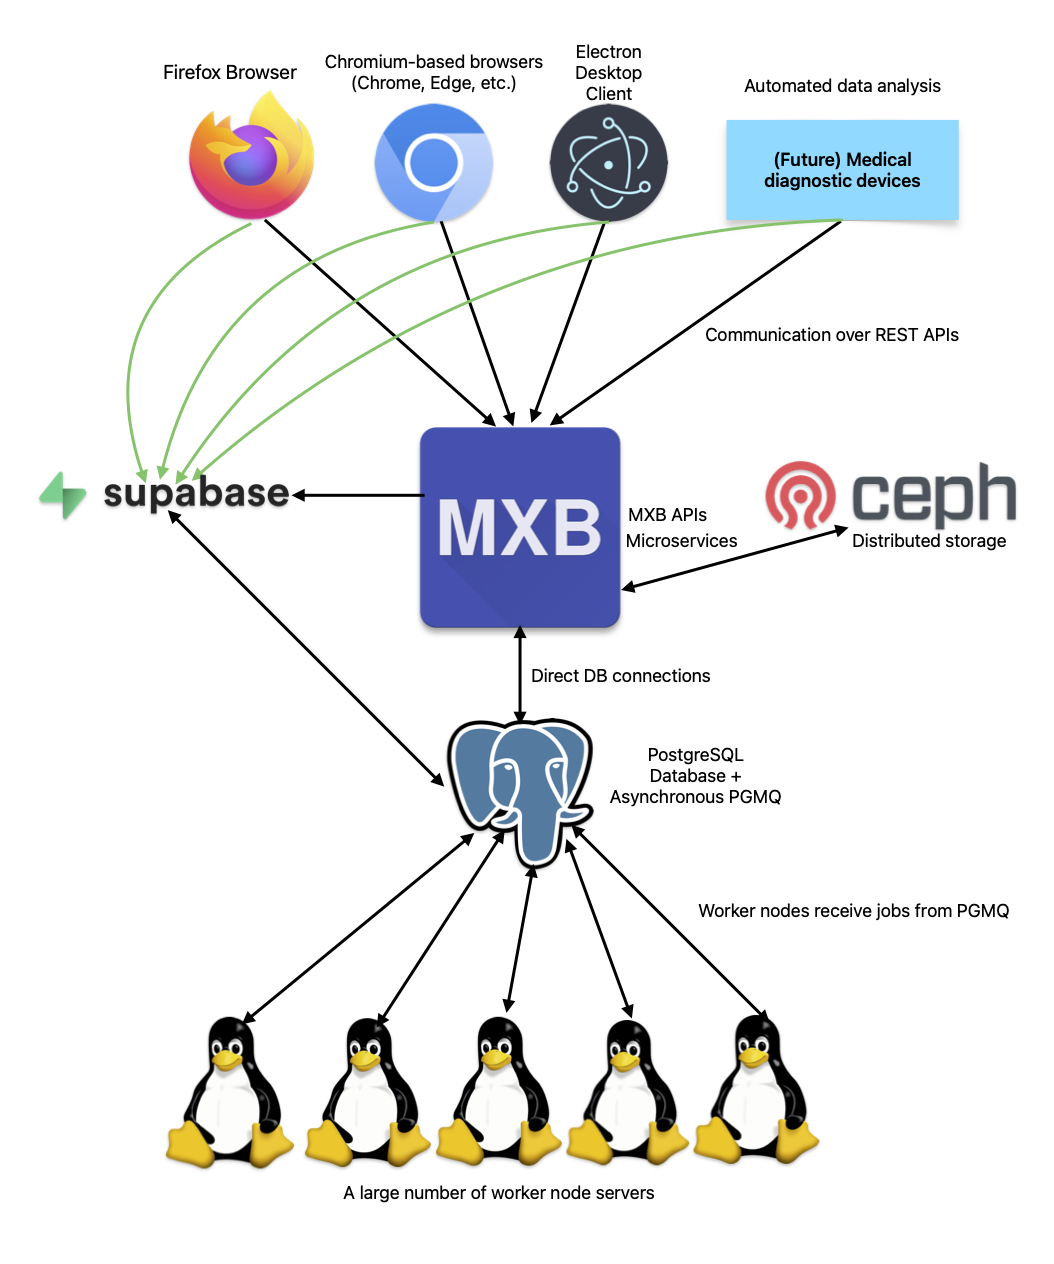
\includegraphics[height=\textheight]{assets/architecture.png}
    \end{figure}
\end{frame}

\begin{frame}{Notable dependencies}
    \begin{figure}
        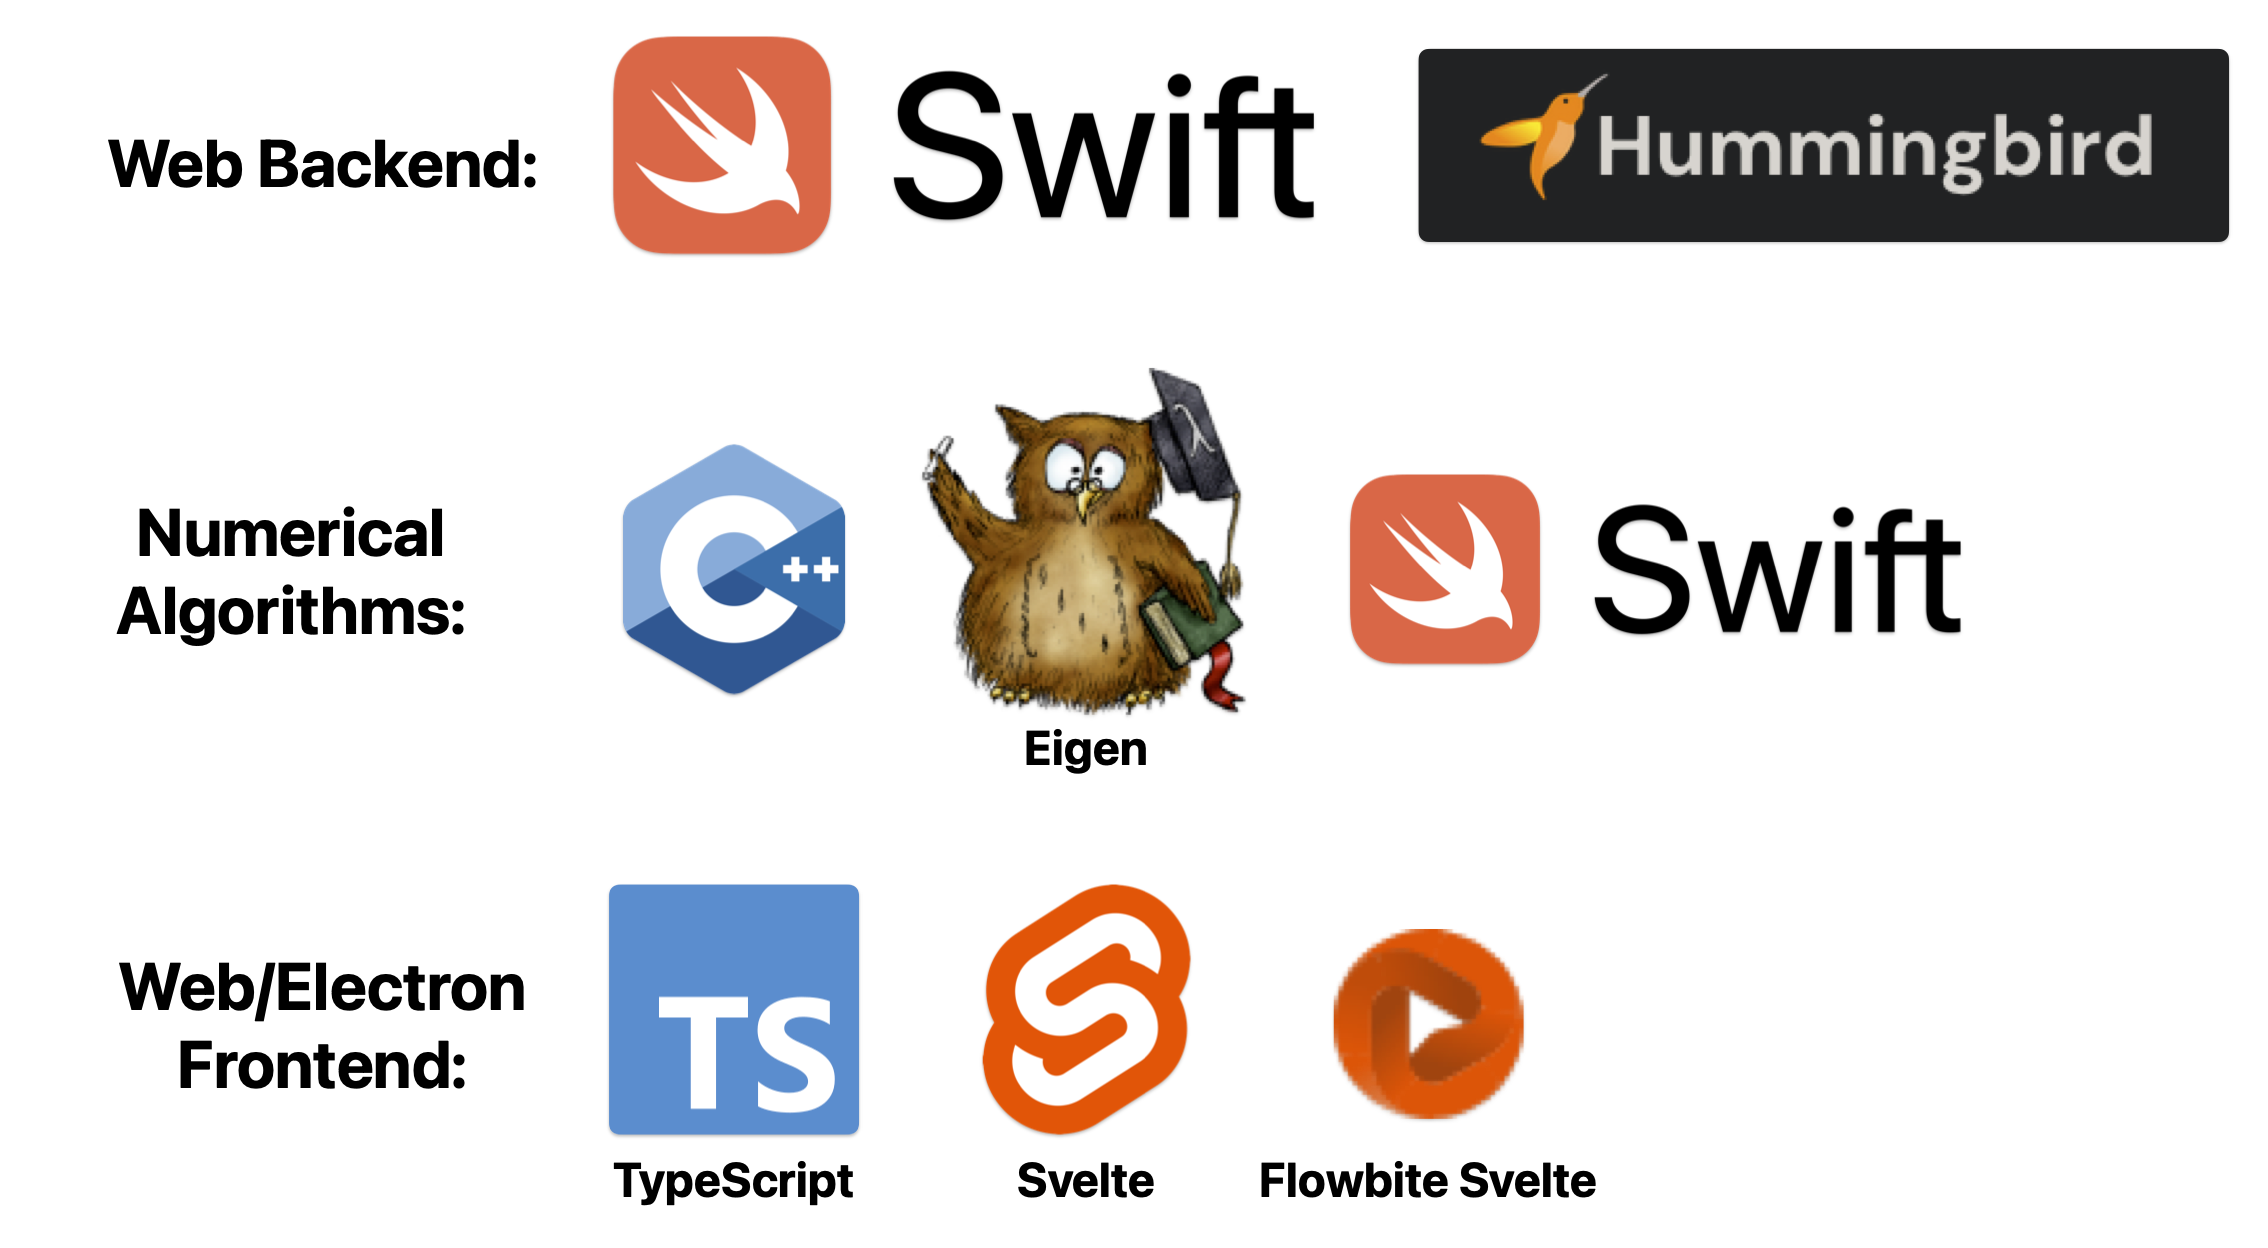
\includegraphics[width=\linewidth]{assets/dependencies.png}
    \end{figure}
\end{frame}

\begin{frame}{One Example Workflow}
    Here, we present a comprehensive, and reproducible machine learning-assisted analysis workflow implemented in MXB.\pause
    \begin{block}{Baseline correction via the algorithm from de Rooi and Eilers.\footnote{\href{https://doi.org/10.1016/j.chemolab.2011.11.001}{Mixture models for baseline estimation, 2012, Johan J.~de Rooi, Paul H.C.~Eilers }}}
        We first fit a mixture model to our experimental current recordings with an expectation-maximization (EM) algorithm. A Gaussian component models the open-pore state signal noise and a uniform component models the blocked-pore state signal. The continuously drifting mean of the Gaussian component is modeled by P-splines, with a $\lambda$ penalization hyperparameter to control for smoothness.
    \end{block}
\end{frame}
    % \framebreak

\begin{frame}{One Example Workflow}

    \begin{block}{Perform thresholding-based blocked-state detection on the standard deviation of the Gaussian distribution from the mixture model}
        For now, we choose to use $3\sigma$ as our blocked-state threshold.
    \end{block}

\end{frame}
    % \framebreak
\begin{frame}{One Example Workflow}
    \begin{block}{Perform thresholding-based event detection on signal during blocked states. }
        Different current levels inside a blocked-pore state's current signal are determined via a newly implemented thresholding algorithm based on the signum of the current signal's finite difference.
        \begin{enumerate}
            \item Segment the signal into maximally long, contiguous intervals for which all sample values' finite differences have the same sign ($+$ or $-$).\pause
            \item The proof for the existence and uniqueness of the segmentation is trivial, and is left to the audience as an exercise.\pause
            \item We define the magnitude of each segment $S$ of length $n$ as $|S| = |S_n| - |S_1|$.\pause
            \item We apply a threshold $\tau$ over the magnitude of each segment to identify new events.
        \end{enumerate}
    \end{block}
    
\end{frame}


\begin{frame}{Computational complexity of the workflow}
    \begin{block}{Matrix multiplications}
        Most of the compute time was spent performing matrix multiplications, which has a complexity of $O(n^3)$ for two square matrices of size $n\times n$. Therefore, algorithmic optimizations and parallel processing are essential to ensure tractability for larger datasets with high sample rates.
    \end{block}\pause

    \begin{block}{Open source \texttt{libpslines}}
        Since the P-Splines baseline estimation algorithm is not specific to the nanopore field, and is of much wider interest to the scientific community, we will open source our high-performance \texttt{libpslines} library separately. It has a \texttt{C}-language binding to ease integration into other projects without requiring \texttt{C++}.
    \end{block}

\end{frame}

\begin{frame}{Computational complexity of the workflow}
    \begin{block}{Optimization compared to de Rooi and Eilers's \texttt{R} implementation for P-spline baseline correction}
        \begin{itemize}
            \item Heartfelt thanks to them for sharing the source code.\pause
            \item Their linear algebra was done with dense matrices, which are not scalable when the data size is large, e.g.~high-sample-rate current recordings. MXB's implementation uses sparse matrices, and implements the algorithm in \texttt{C++} with \texttt{Eigen} to achieve significant performance improvement.
        \end{itemize}
    \end{block}
\end{frame}

\begin{frame}{Computational complexity of the workflow}
    \begin{block}{Optimization compared to de Rooi and Eilers's \texttt{R} implementation for P-spline baseline correction}
        They implemented the M step of EM algorithm by solving for the Moore-Penrose pseudoinverse of a potentially-large matrix, which can be an $O(n^3)$ operation depending on different library implementations. We improve the performance by using a solver for the linear system of equations based on complete orthogonal decomposition, which is cheaper to compute than singular value decomposition. Our chosen solver has a time complexity of $O(n^2)$.
    \end{block}
\end{frame}

\begin{frame}{Computational complexity of the workflow}
    The thresholding steps have a complexity of $O(n)$. As expected, the cubic-time operation of matrix multiplication asymptotically dominates.\pause
    \begin{block}{Algorithms of $O(n^3)$ complexity are classically considered intractable. So, what do?}
        Parallelism to the rescue!\\\vspace{3mm}
        \begin{figure}
            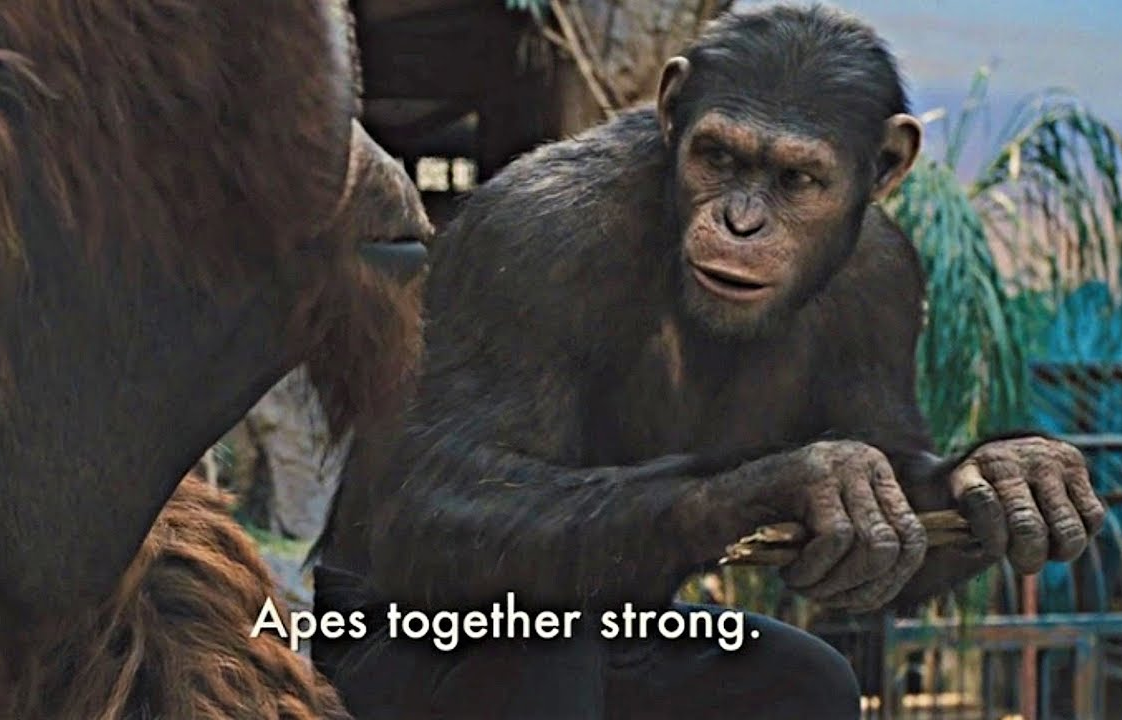
\includegraphics[width=5cm]{assets/apes.png}
            \caption{Rise of the Planet of the Apes, 2011 \href{https://www.imdb.com/title/tt1318514/}{\texttt{https://www.imdb.com/title/tt1318514/}}}
        \end{figure}
        
    \end{block}
\end{frame}


\begin{frame}{Scatter-gather parallel processing for each experimental recording}
    \begin{figure}
        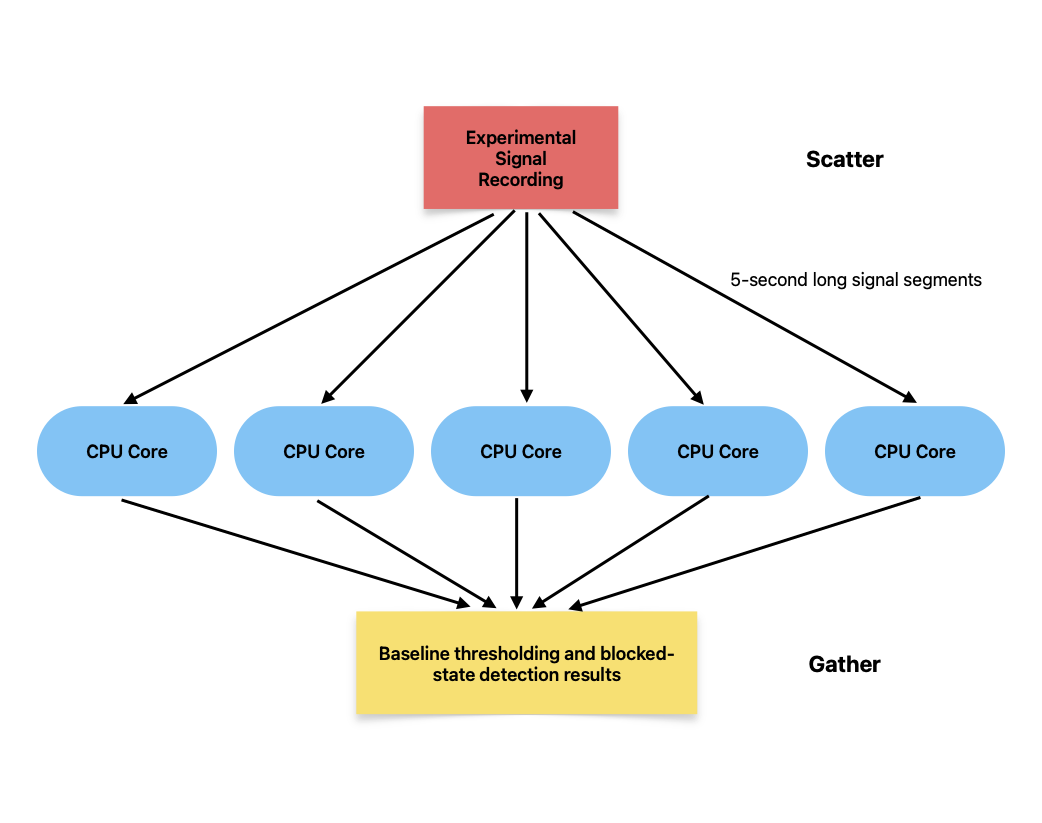
\includegraphics[width=\linewidth]{assets/scatter-gather-recording.png}
    \end{figure}
\end{frame}

\begin{frame}{Scatter-gather parallel processing over a set of recordings}
    \begin{figure}
        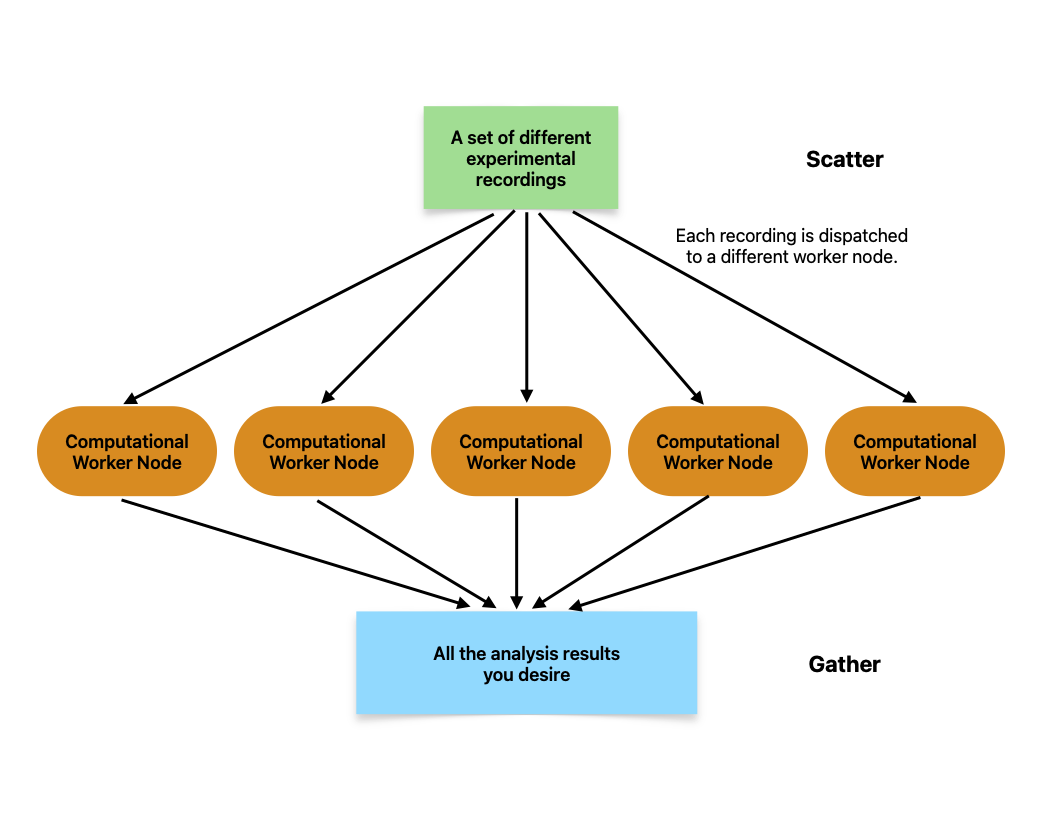
\includegraphics[width=\linewidth]{assets/scatter-gather-files.png}
    \end{figure}
\end{frame}

\begin{frame}{SIMD performance for signal processing}
    \begin{block}{SIMD (Single-instruction, multiple data)}
        \begin{itemize}
            \item On AMD64, AVX-512 is important to achieve good performance. Even at lower memory clocks, the Ryzen 5 7700 from AMD is better than the Intel Core i9-13900K in single-core performance.\pause
            \item On Apple Silicon (2025 MacBook Pro with M4 Max), the CPU-only performance is comparable to CUDA. Unclear if it is the result of the ARM architecture, Apple's M-series microarchitecture, or faster memory access on an SoC.\pause
            \item NVIDIA's CUDA is fast and achieves reliable real-time processing of incoming data, but expensive. An array of Mac Minis are likely to be fast enough while being much more cost effective.
        \end{itemize}
    \end{block}
\end{frame}

\begin{frame}[allowframebreaks]{Why is CUDA not faster than Apple Silicon CPUs}
    \begin{block}{CUDA's priority for low-precision arithmetics}
        CUDA has been optimized for deep learning and in particular, LLM training, which benefits from low-precision floating point arithmetics, such as \texttt{f16}, \texttt{bf16}, or even \texttt{int8}. However, our implementation of de Rooi and Eilers's EM algorithm occasionally fails to converge with single-precision floating point numbers (f32), due to accumulated errors.
    \end{block}\pause

    
    \begin{block}{Then, why not use a different baseline estimation method?}
        Other methods such as asymmetric least square smoothing and their improved versions are not optimized for excluding long-lasting blocked-state signals in the baseline.
    \end{block}
\end{frame}

\begin{frame}{What makes \texttt{MXB} awesome?}
    \begin{itemize}
        \item Easily reproducible analysis results. It would be a boon to the field to make reproducibility a requirement for publication of new papers.\pause
        \item No need to purchase expensive computers. It's cheaper for everyone to pool resources together in cooperation.\pause
        \item The analysis pipelines your develop can be operationalized into medical diagnostic devices effortlessly, and without requiring expensive custom computing hardware built into diagnostic devices themselves.\pause
        \item Free and open source, benefitting the entire nanopore community. We welcome and invite your participation and contribution, including code contributions and bug reports.
    \end{itemize}
\end{frame}

\begin{frame}{Free as in freedom! \texttt{MXB}'s beta release}
    \begin{itemize}
        \item The source code will be available on \url{https://codeberg.org/}, and mirrored to GitHub.
        \item Due to resource limitations, we cannot serve too many users at the beginning. If you are interested in using MXB during our beta release, please send me an email at: \href{mailto:catherine@catherinexiao.com}{catherine@catherinexiao.com}.
        \item Disclaimer: the common \texttt{.abf} files are a secretive, and non-standardized proprietary software format. Your files are likely might not be readable by MXB. But we consider this a bug, and will endeavor to provide fixes. Please file a bug report on Codeberg in such cases. Furthermore, we plan to package our ABF reader separately as \texttt{libabf}, if there is community demand.
    \end{itemize}
\end{frame}

\begin{frame}{Linus's Law, or the Cathedral and the Bazaar}
    \begin{quotation}
        Given enough eyeballs, all bugs are shallow.\\
        -- Eric S.~Raymond~\footnote{\href{http://www.catb.org/~esr/writings/cathedral-bazaar/}{The Cathedral and the Bazaar, 1999, Eric S.~Raymond}}
    \end{quotation}

    Please join us in making buggy software a thing of the past in this cluster.\footnote{This presentation is free and open source under the GNU AGPL license, and you may find the source code \href{https://github.com/cathxiao/presentation-nanodiag-2025}{on GitHub}.}
\end{frame}

\begin{frame}{Many thanks for making \texttt{MXB}'s open source release possible}
    \pause
    \begin{block}{Thank you! May your software be forever free and open source, and receive blessings from Saint IGNUcius (Richard Stallman) of the Church of Emacs.}
        \begin{figure}
            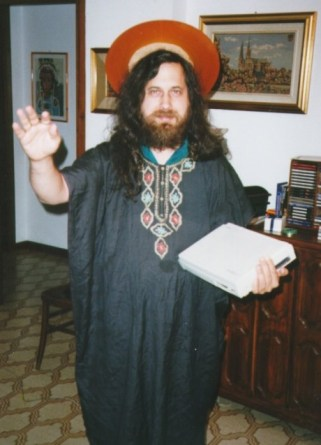
\includegraphics[height=4cm]{assets/saintignucius.jpg}
            \caption{There is no operating system but \texttt{GNU}, and \texttt{Linux} is one of its kernels.
            \href{https://www.stallman.org/saint.html}{https://www.stallman.org/saint.html}}
        \end{figure}
    \end{block}
    
\end{frame}

\end{document}
